% Auf ungerader Seite starten
\cleardoublepage

\chapter{Results}
\label{Chapter:Results}

%\section{Prediction Perfomance of Models}

\section{Verification of FI algorithms}
Before applying the eight feature importance methods to the C-MAPSS models, a controlled verification experiment was carried out to confirm that the implementations behave as expected when ground truth is known. The idea is simple: train a model where the true feature importances are unambiguous, then check whether each method recovers them.

The setup uses a linear function of tn input variables:
%
\begin{equation}
    f(x) = 5x_0 + 3x_1 + 2x_2 +1.5x_3 + 1X_4 + 0x_5+ 0x_6+ 0x_7+ 0x_8+ 0x_9
\end{equation}
%
The first five features carry all the predictive information, with known weights of 5, 3, 2, 1.5 and 1. The remaining five features ($x_5$ through $x_9$) have zero weight, they are pure noise. A single-layer linear neural network without activation functions was trained on 4000 samples drawn from a unifrom distribution over [0, 10]. After training, the learned weights matched the true weights to four decimal places, confirming that the model itself was not a source of error.

All eight feature importance methods were then applied to the trained model using the test set. The resulting attributions were scaled to compare true weights with the trained weights, allowing a direct comparison. \ref{fig:golden_test} shows the results.

\begin{figure}[h]
    \centering
    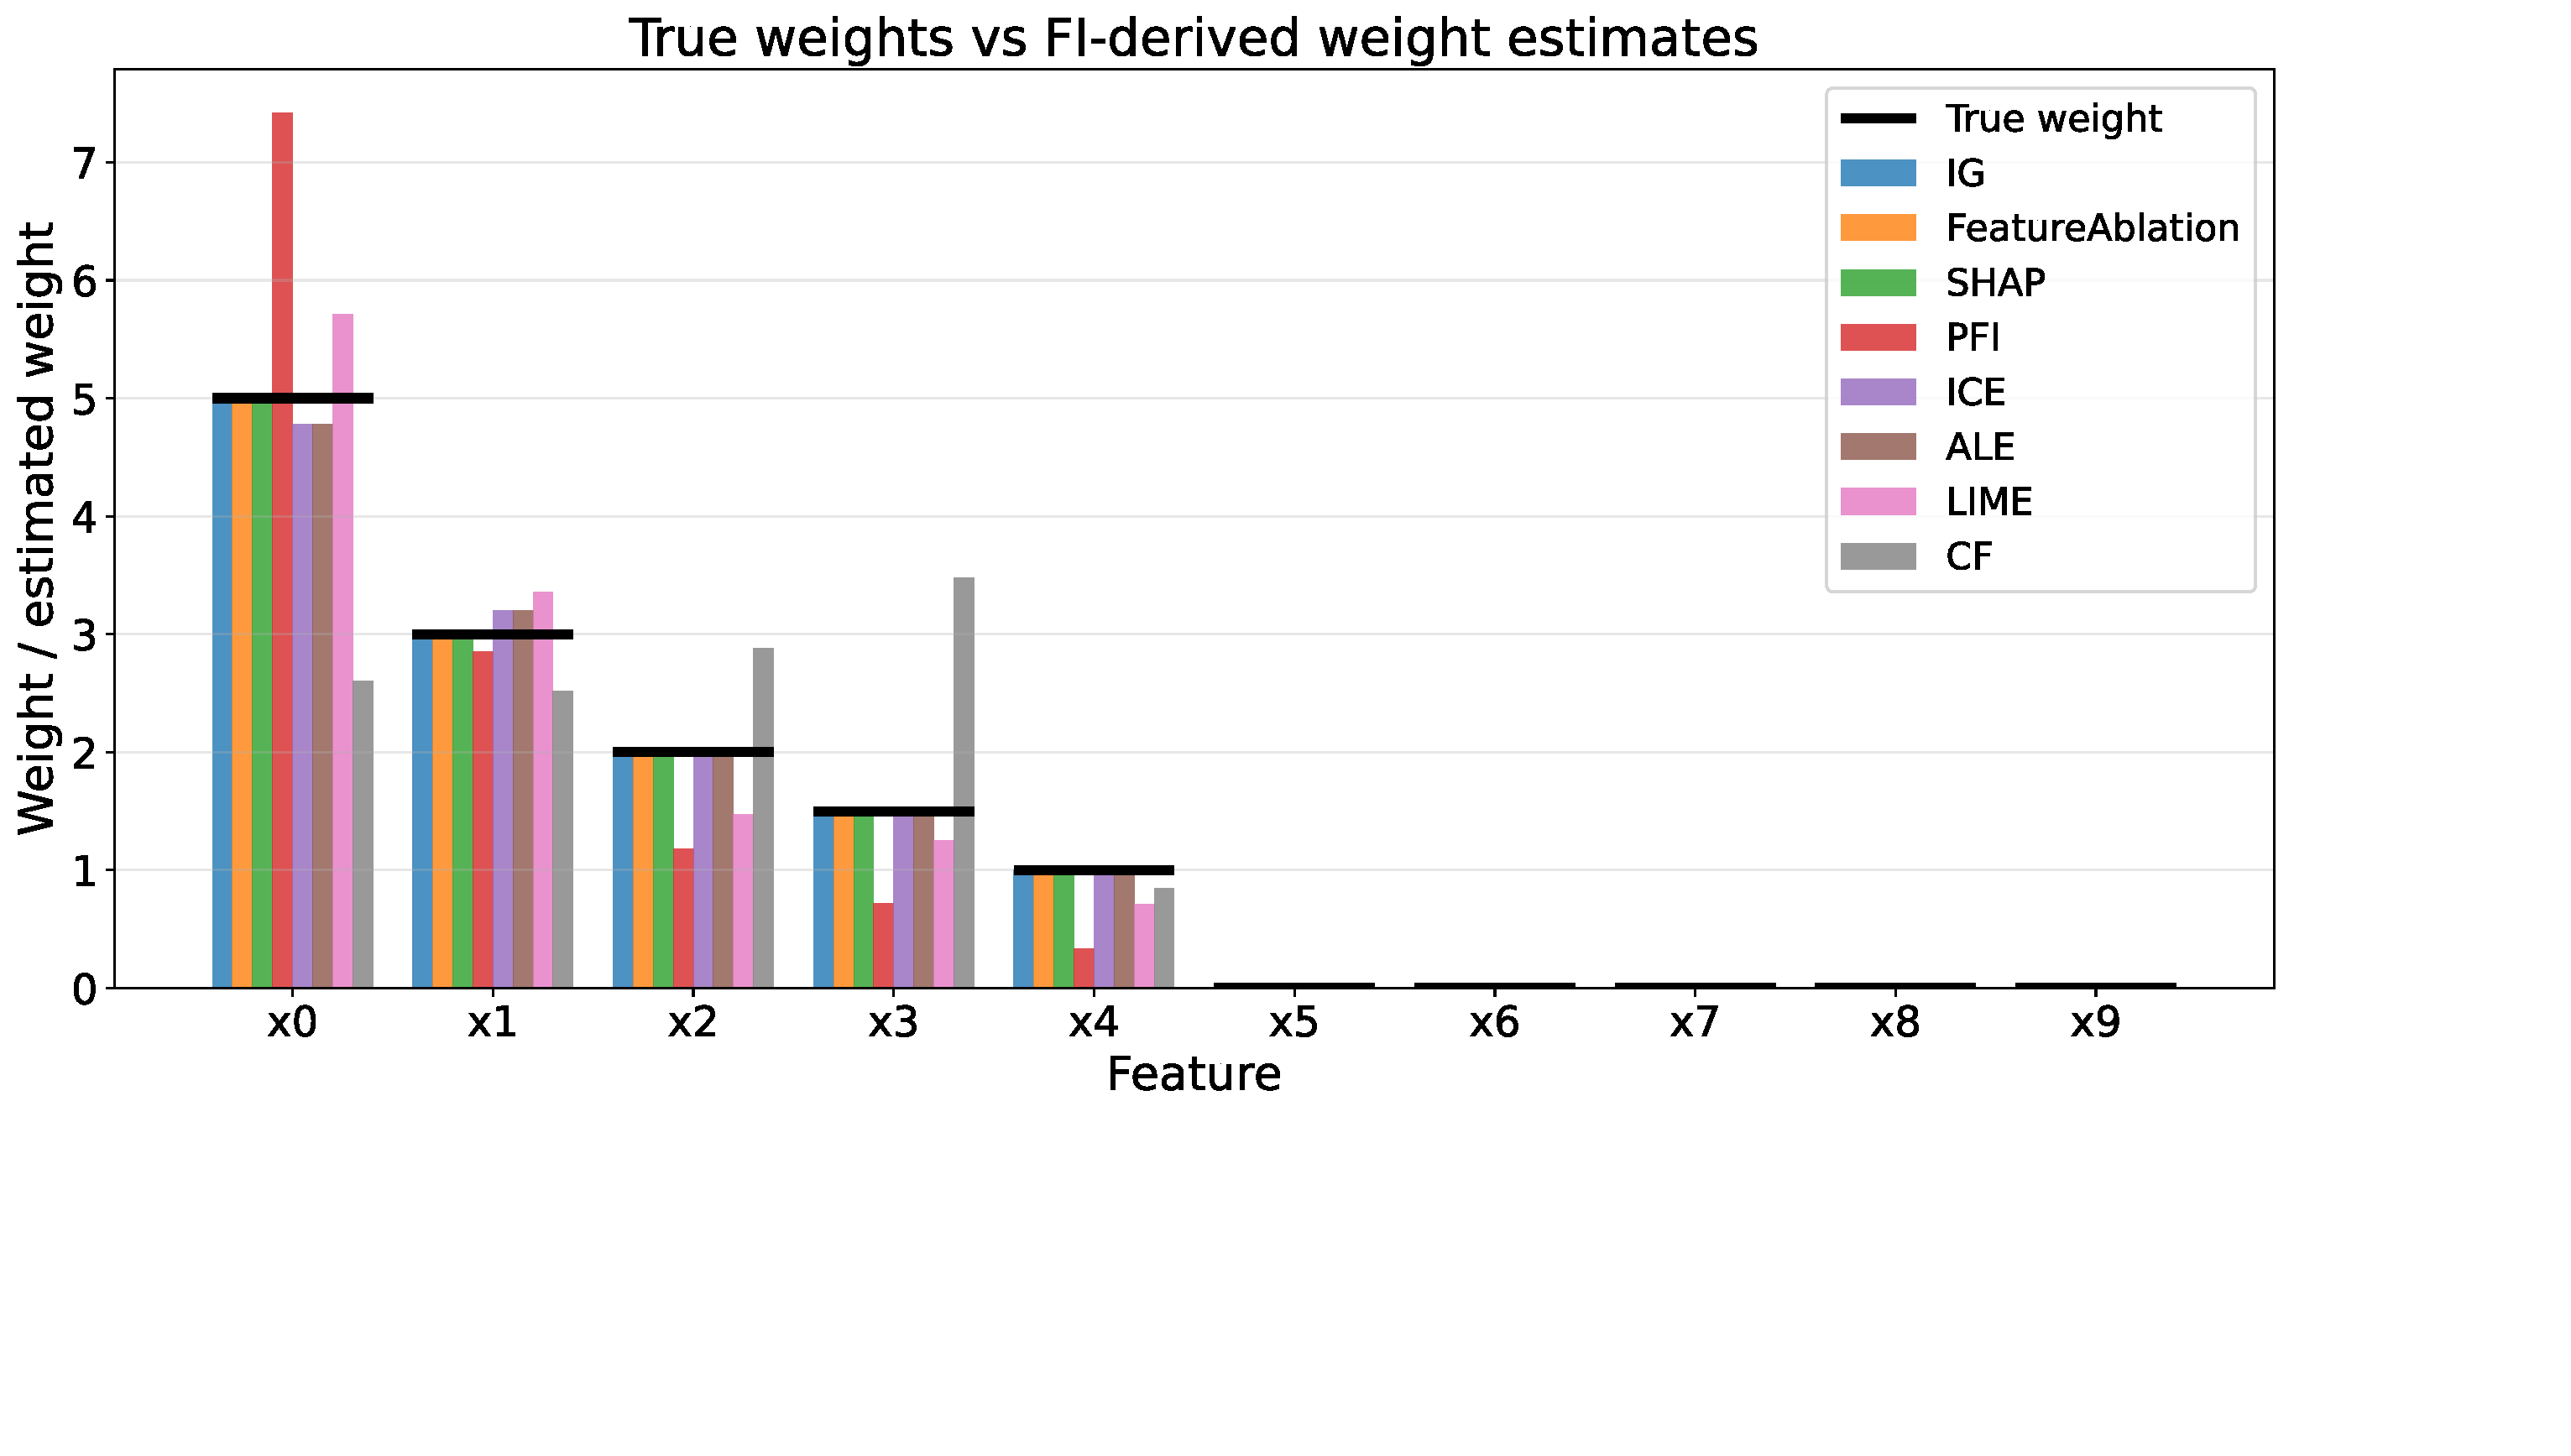
\includegraphics[width=\textwidth]{bilder/Results/golden_test_weights.pdf}
    \caption{Verification of feature importance implementations on a linear model with known weights. Bars show estimated weight; black markers indicate the true weights.}
    \label{fig:golden_test}
\end{figure}

Six of the eight methods, Integrated Gradients, Feature Ablation, SHAP, ALE, ICE and LIME, cloesly reproduce the true weight distribution. Their bars track the ground truth across all ten features, correctly assigning near-zero importance to $x_5$ through $x_9$ and recovering the correct ranking and approximate magnitudes for $x_0$ through $x_4$. Minor deviaitons exist, ICE slightly overestimates the importance of $x_0$ relative to the other active featrues, but these are within the range expected from sampling variability.

Permutation Feature Importance (PFI) and Counterfactual Explanations (CF) show larger deviations, thugh for different reasons.

PFI overestimates $x_0$ substantially, roughly 2.5 in estimated weight terms, versus the true value of 5, while compressing the remaining active features downward. The ranking among $x_0$ through $x_4$ is preserved and $x_5$ through $x_0$ are correctly identified as irrelevant. The skew toward $x_0$ is a known property of PFI on correlated or hgih-variance features: because PFI measures the increase in prediction error when a feature is permuted, the feature with the largest absolute weight causes the largest error disruption when shuffled, and this effect scale nonlinearly with the weight magnitude under squared-error metrics like MSE. The relative ordering is correct, but the magnitdue distribution does not directly reflect the underlying weight ratios.

Counterfactual Explanations show a different kid of deviation. Rathern than preserving the ranking with distorted magnitudes, CF partially msorders the active features, in the raw weieght estimates, $x_3$ receives the highest estimated weight and the overall distribution across $x_0$ through $x_4$ does not follow the true ordering . This is not unexpected. Counterfactual methods search for the smallest input change that shifts the prediction into a target range. That search depends on the local geometry of the predictino surface and the permitted perturbation ranges, not directly on the magnitude of learned weights. In a linear model the prediction surface is uniformly sloped, which removes the kind of local structure that counterfactual search id designed to exploit, making this an inherently unfavourable test case for the method. On more complex models with nonlinear interactions, such as the 1D CNN used on C-MAPSS, counterfactual explanations may behave more meaningfully.

The key outcome of this verification is that all eight methods correctly distinguish relevant feature from irrelevant ones. The six gradient-based, perturbation-based and marginal-effect methods additionally recover the correct rankin and approximate magnitudes. PFI recovers the ranking but distorts magnitudes. CF struggles with both ranking and magnitudes on this liinear test case, but still separates the two groups cleanly. These results provide confidence that the implementation are functioning correlcy and that observed differences on C-MAPSS reflect genuine properties of the methods rather than implementation errors.

\section{Individual Method Results}
Before comparing the eight methods against each other, it is worth looking at the kind of output they produce individually. This section shows representative ICE curves and SHAP plots, all from the single-FD001 model, the simplest configuration and therefore the easiest to interpret. Complete plots for all model configurations are provided in Appendix \ref{app:individual_results}

\subsection{ICE Curves}
ICE plots show how the model's RUL prediction changes as a single sensor value is varied across its oberved range, with one curve per test instance. The black line is Partial Dependence (PD) curve, the average across all instances.
%
\begin{figure}
    
\end{figure}
%
For s9, the individual ICE curves spread across a range of roughly $\pm 0.4$ in centered RUL, with several raching $\pm 0.6$ or beyond at the extremes of the sensor range. The PD curve shows a mild negative trend, higher s9 values are associated with slightly lower predicted RUL, but the more telling aspect is the spread itself. The wide dispersion of individual curves mean that the effect of s9 on the prediction depends heavily on the values of the other sensor for that particular engine instance. The model is not using s9 in a simple, unifrom way; its influence interacts with the broader sensor context.

\begin{figure}
    
\end{figure}

Sensor s3 looks entirely different. The PD curve is effectively flat and the individual ICE curves are tightly clustered within $\pm 0.1$. Varying s3 across its full range barely moves the prediction regardless of context. The model has learned to largely ignore this sensor, consistent with the comparative importance rankings in the next section, where s3 appears near the bottom across all methods.

The contrast between these two sensors illustrates what ICE curves are goot ad: they do not just say "this sensor matters more than that one," they show \textit{how} a sensor's effect manifests, whether it is roughly unifrom across instances or highly variable, suggesting interactions with other features.

\subsection{SHAP Analysis}
Figure ~\ref{fig:shap_beeswarm} shows the SHAP beeswarm plot for the single-FD001 model. Each dot represents one test instance; horizontal position indicates the SHAP value (contribution to the prediction) and colour indicates the sensor reading for that instance (red for high, blue for low).
%
\begin{figure}
    
\end{figure}
%
Sensor s9 stands out immediately, it has by far the widest spread of SHAP values, ranging from approximately $-0.5$ to $+0.3$. No other sensor comes close in magnitude. Sensors s4 and s1 form a second tier, with SHAP values reaching roughly $\pm 0.2$. The remaining sensors cluster much more tightly around zero, contributing little to individual predictions. The colour gradient reveals directional effects: for s4, blue dots (low sensor values) tend to produce positive SHAP values and red dots (high values) tend to push negative, meaning that as s4 increases, the modell predicts lower RUL. Sensors further down the ranking, s17 and s3, show very narrow SHAP distributions, confirming that the model assigns them minimal influence on this subset.

Figure ~\ref{fig:shap_waterfall} shows a SHAP waterfall plot for asingle test instance, breaking down how the model moves from the expected prediction $E\left[f(X)\right] = 0.007$ to the instance-specific prediction $f(x)=0.265$.

\begin{figure}
    
\end{figure}
Sensor s9 accounts for almost the entire deviation, contributing $+0.23$, roughly 90\% of the shift from the baseline. Sensor s2 adds another $+0.12$ and the remaining sensors contribute small positive or negative adjustments that partially cancel each other. The waterfall makes visible what the beeswarm shows statistically: onn this model, s9 is the dominant drive of individual predictions and most other sesnros play a supporting or corrective role.

The SHAP plots add directional informatino that the bar chart comparisons in the next section cannot provide. Where the bar charts show \textit{how much} each sesnor matters in aggregate, the beeswarm and waterfall show in \textit{in which direction} and \textit{for which instances}, whether a high sensor reading pushes predicted RUL up or down. This directional detail is useful for sanity-checking the model against physical expectations, a point returnde to in the Discussion.

\section{Comparative Feature Importance Across Methods}
The core of this analysis is the side-by-side comparison of all eight methods on the same model and dataset. Each figure shows L1-normalised sensor importance from every method, with sensors ordererd by decreasing average importance. Four representative configurations are shown: models trained on FD001 alone, FD002 alone, the FD001-FD002 pair, and all four subsets combined. Remaining configurations are included in Appendix~\ref{app:comparative_results}.

\subsection{Single-Dataset Models}
\begin{figure}[ht]
    \centering
    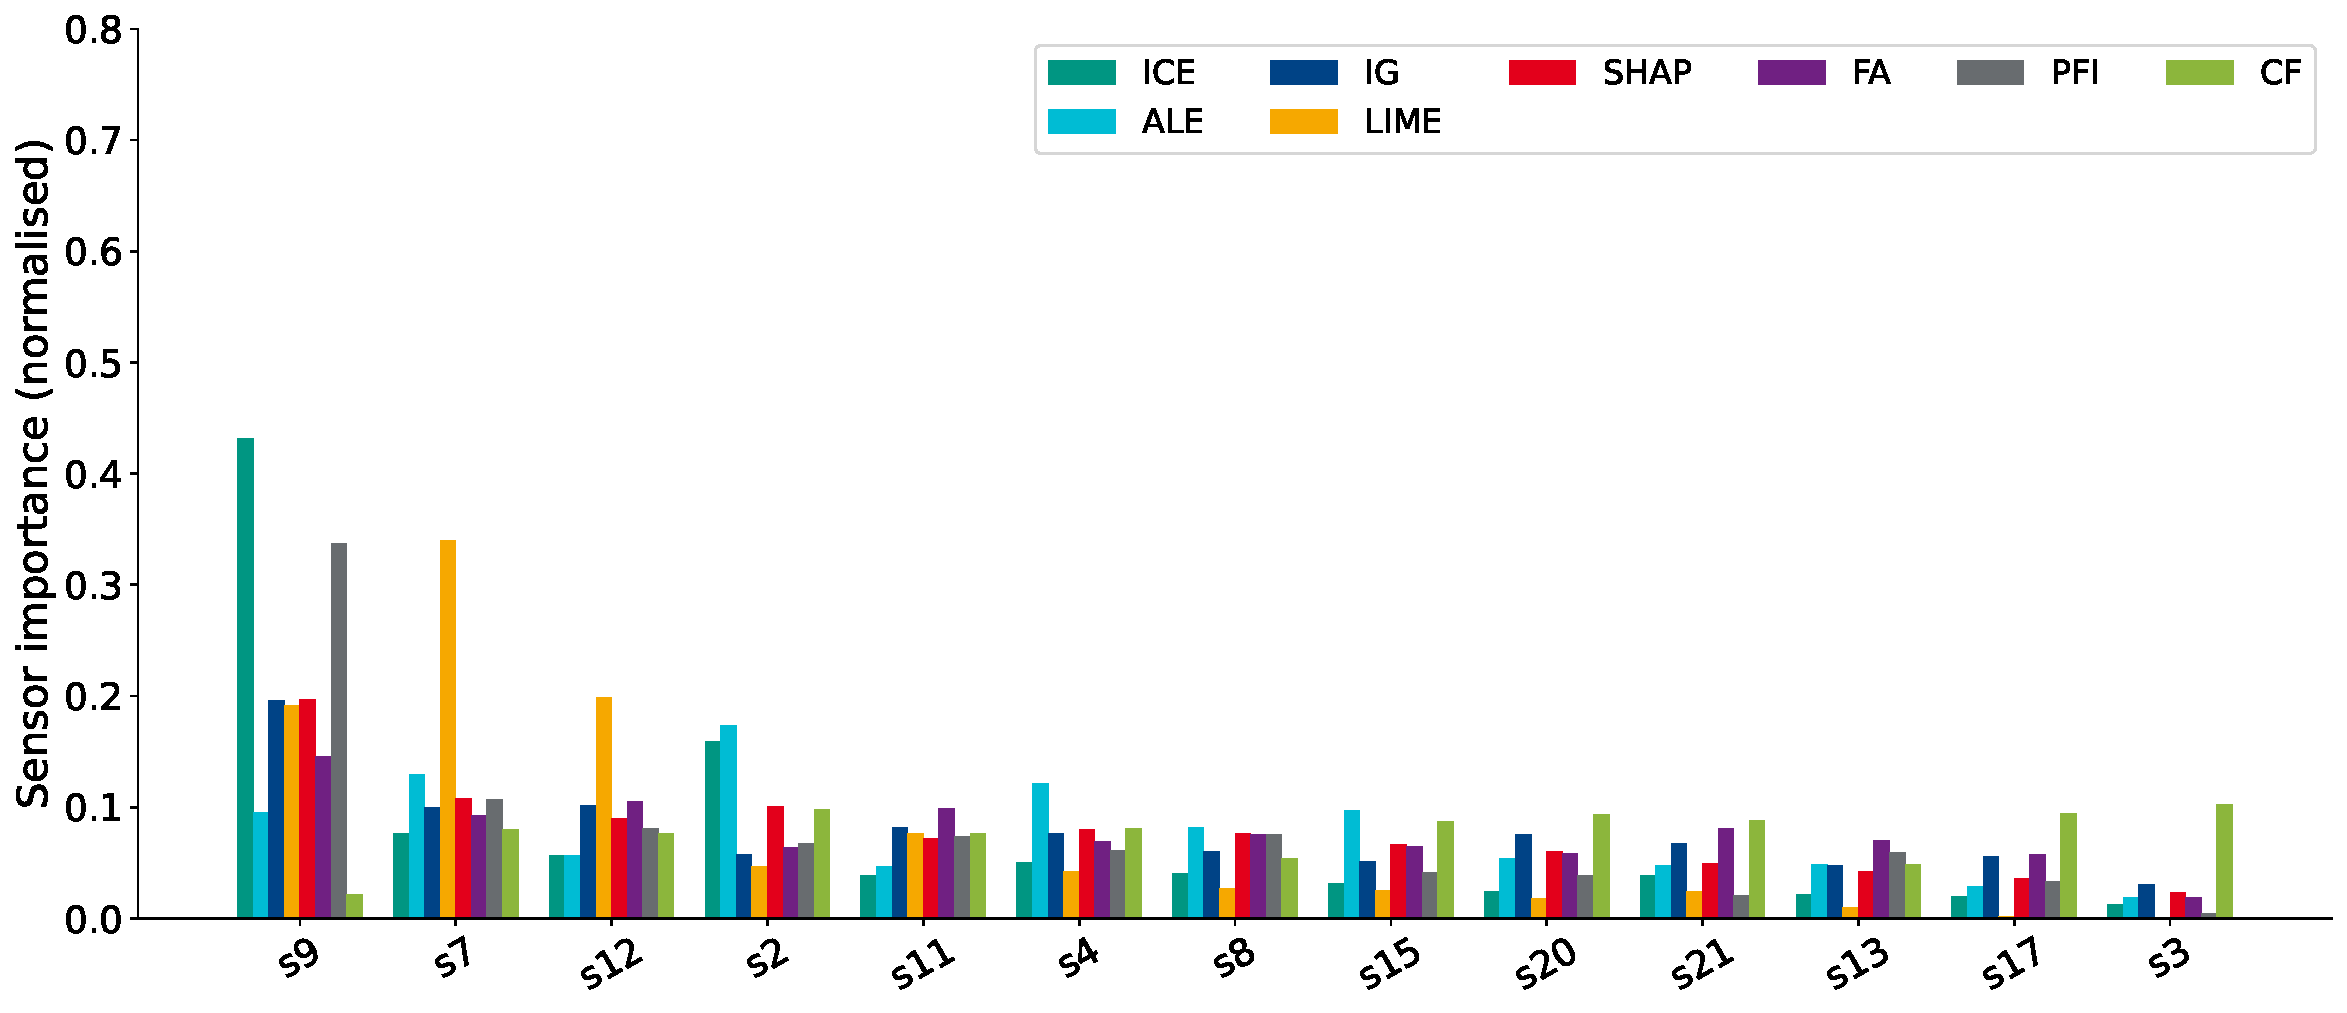
\includegraphics[width=\textwidth]{bilder/Results/compare_methods_single_FD001.pdf}
    \caption{L1-normalised sensor importance across all eight methods for the single-FD001 model. Sensors are ordered by decreasing mean importance.}
    \label{fig:compare_FD001}
\end{figure}

On the single-FD001 model, s9 is the most important sensor according to most methods. ICE assigns it roughly 0.43, PFI around 0.34, and the gradient- and perturbation-based methods (IG, SHAP, FA) converge around 0.19-0.20. The next tier, s7, s12, and s2, is where methods start to diverge. LIME assigns s7 a normalised importance of roughly 0.34, well above what the other methods give it. ALE places s12 and s4 higher than most alternative. The broad picture is consistent though: s9 leads, a group of four or five sensors follows with moderate importance and the remainder contributes little.

\begin{figure}[ht]
    \centering
    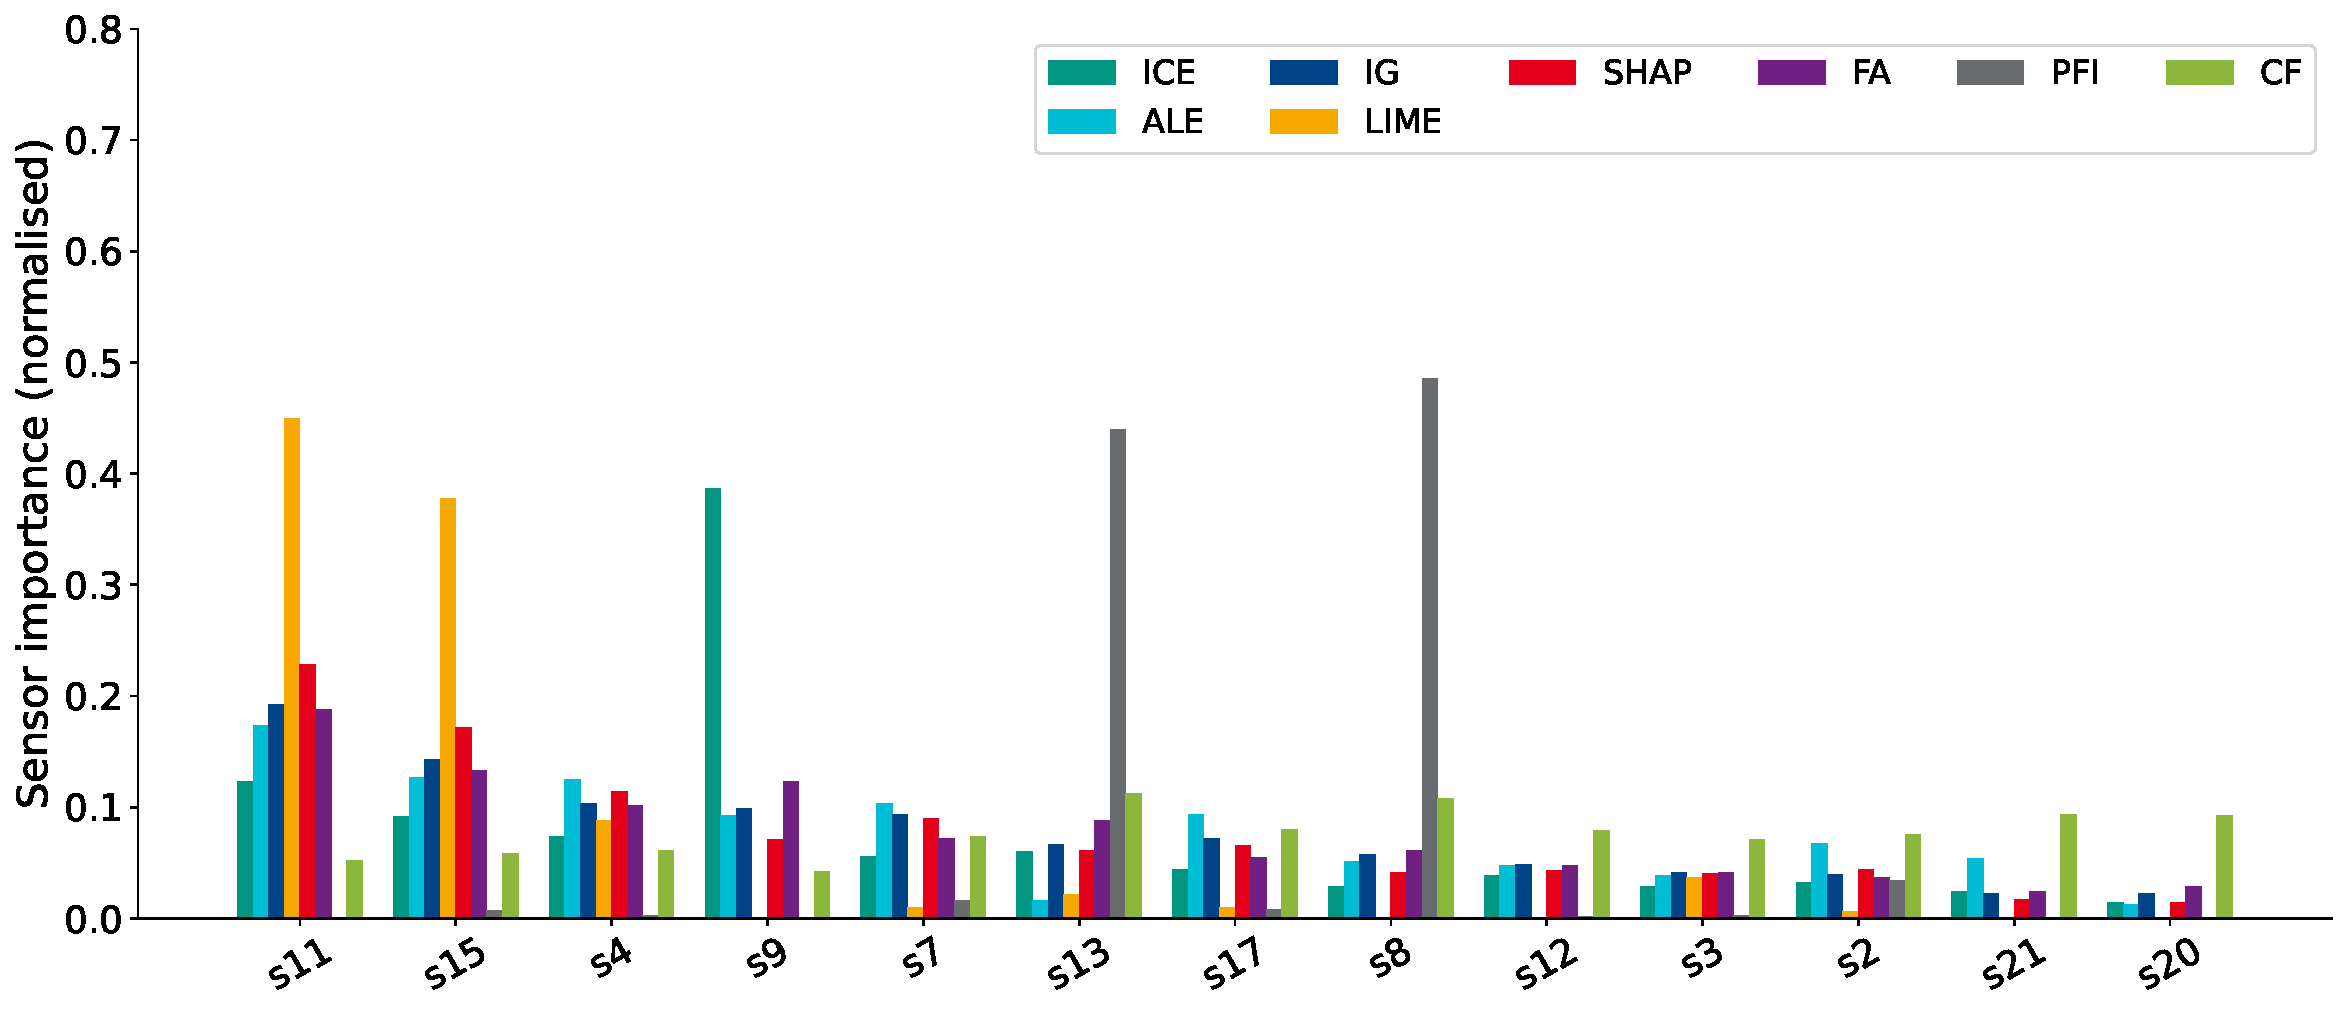
\includegraphics[width=\textwidth]{bilder/Results/compare_methods_single_FD002.pdf}
    \caption{L1-normalised sensor importance across all eight methods for the single-FD002 model. Sensors are ordered by decreasing mean importance.}
    \label{fig:compare_FD002}
\end{figure}

FD002 changes the picture substantially. With sixx operating conditions instead of one, the model faces more complex input distributions and snsor rankings shift accordingly. Sensor s11 emerges as the most important for IG, ALE, SHAP and FA, the four methods that tended to agree most closely on FD001 as well. LIME concentrates even more aggressively, assigning s11 roughly 0.45 and s15 around 0.38, leaving little importance for anything else. PFI produces extreme outlier spikes, s8 receives nearly 0.49 and s13 around 0.44, not reflected by any other method. These PFI spikes are reminiscent of the magnitude distortion observed in the verification experiment and suggest that PFI's MSE-based scoring amplifies the apparent importance of features whose permutation causes large error in isolated instances.

ICE remains erratic in regards to assigning s9 the highest importance at around 0.39 while other methods rank it considerably lower.

\subsection{Multi-Dataset Models}
\begin{figure}[ht]
    \centering
    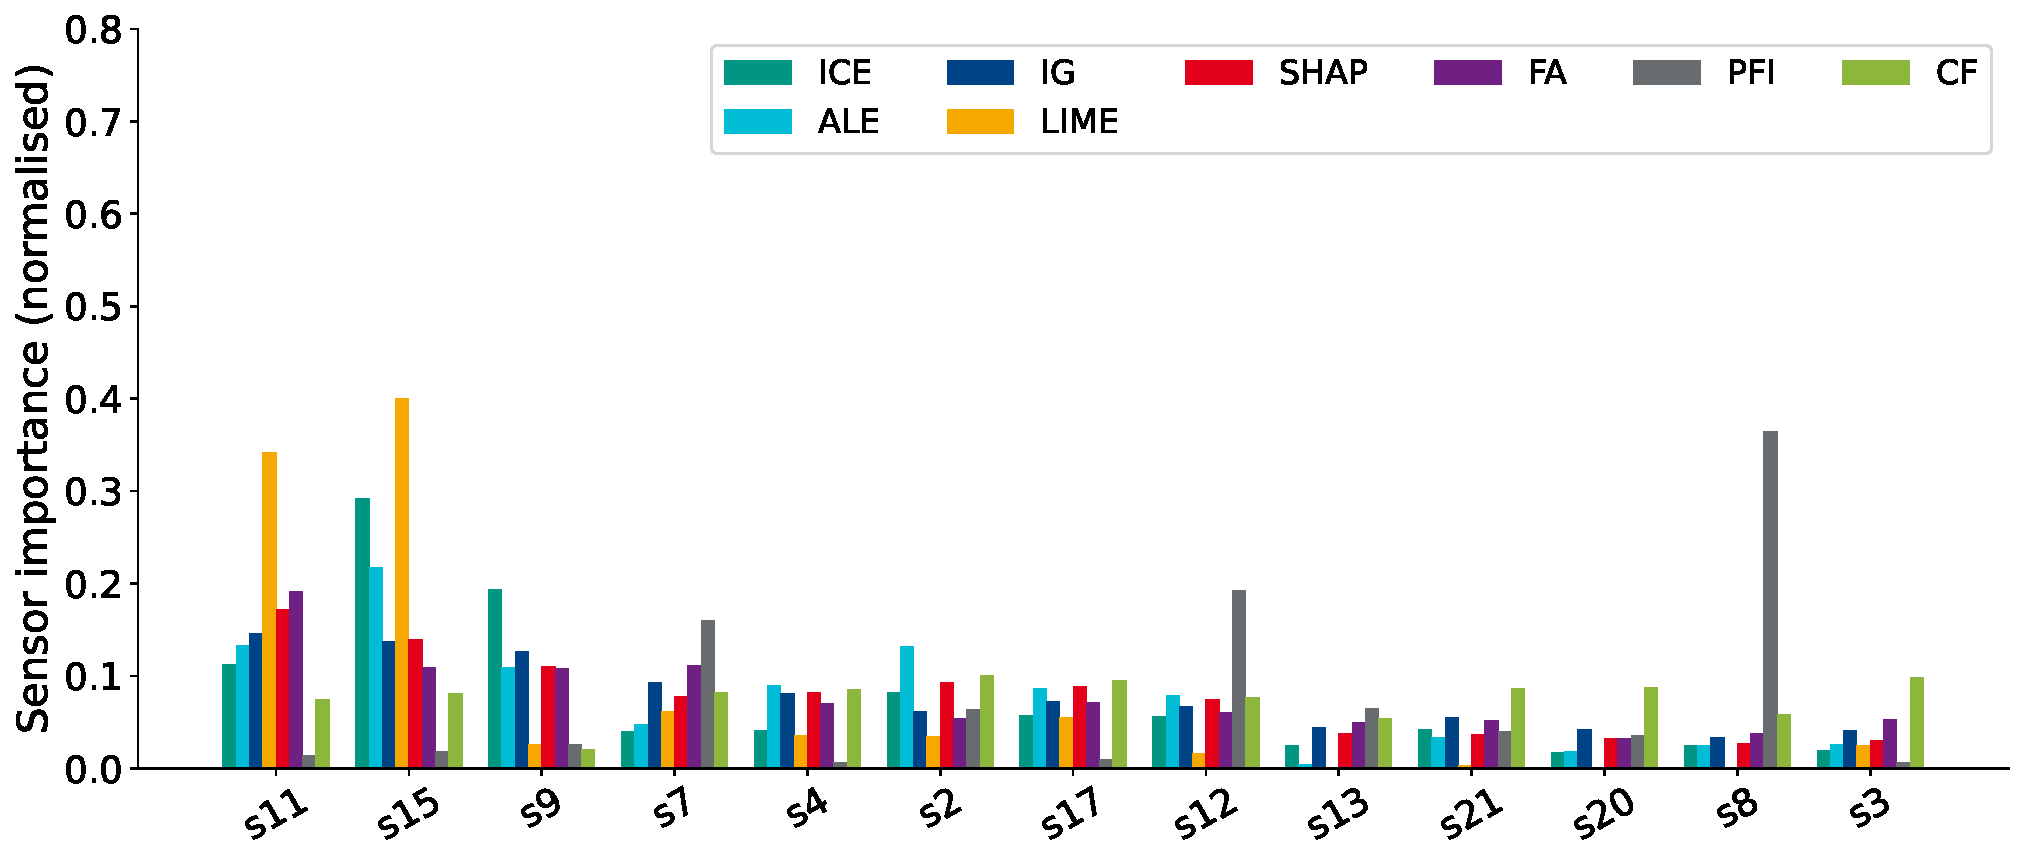
\includegraphics[width=\textwidth]{bilder/Results/compare_methods_pairwise_FD001_FD002.pdf}
    \caption{L1-normalised sensor importance across all eight methods for the pairwise-FD001-FD002 model. Sensors are ordered by decreasing mean importance.}
    \label{fig:compare_FD001_FD002}
\end{figure}

When the model is trained on FD001 and FD002 together, the rankings stabilise somewhat. Sensors s11 and s15 emerge as the top two across most methods, with s9, s7 ands4 forming a second tier. The pairwise model has seen both single-condition and multi-condition data and the resulting importance reflects a compromise: sensors that dominated under one condition (s0 for FD001, s11 for FD002) bot retain importance, but neither dominates as strongly as it did alone. PFI still produces an isolated spike on s8 ($\sim0.36$), unsupported by any other method. LIME remains heavily concentrated on s11 and s15, allocating aaround 0.35 and 0.40 respectively.

\begin{figure}[ht]
    \centering
    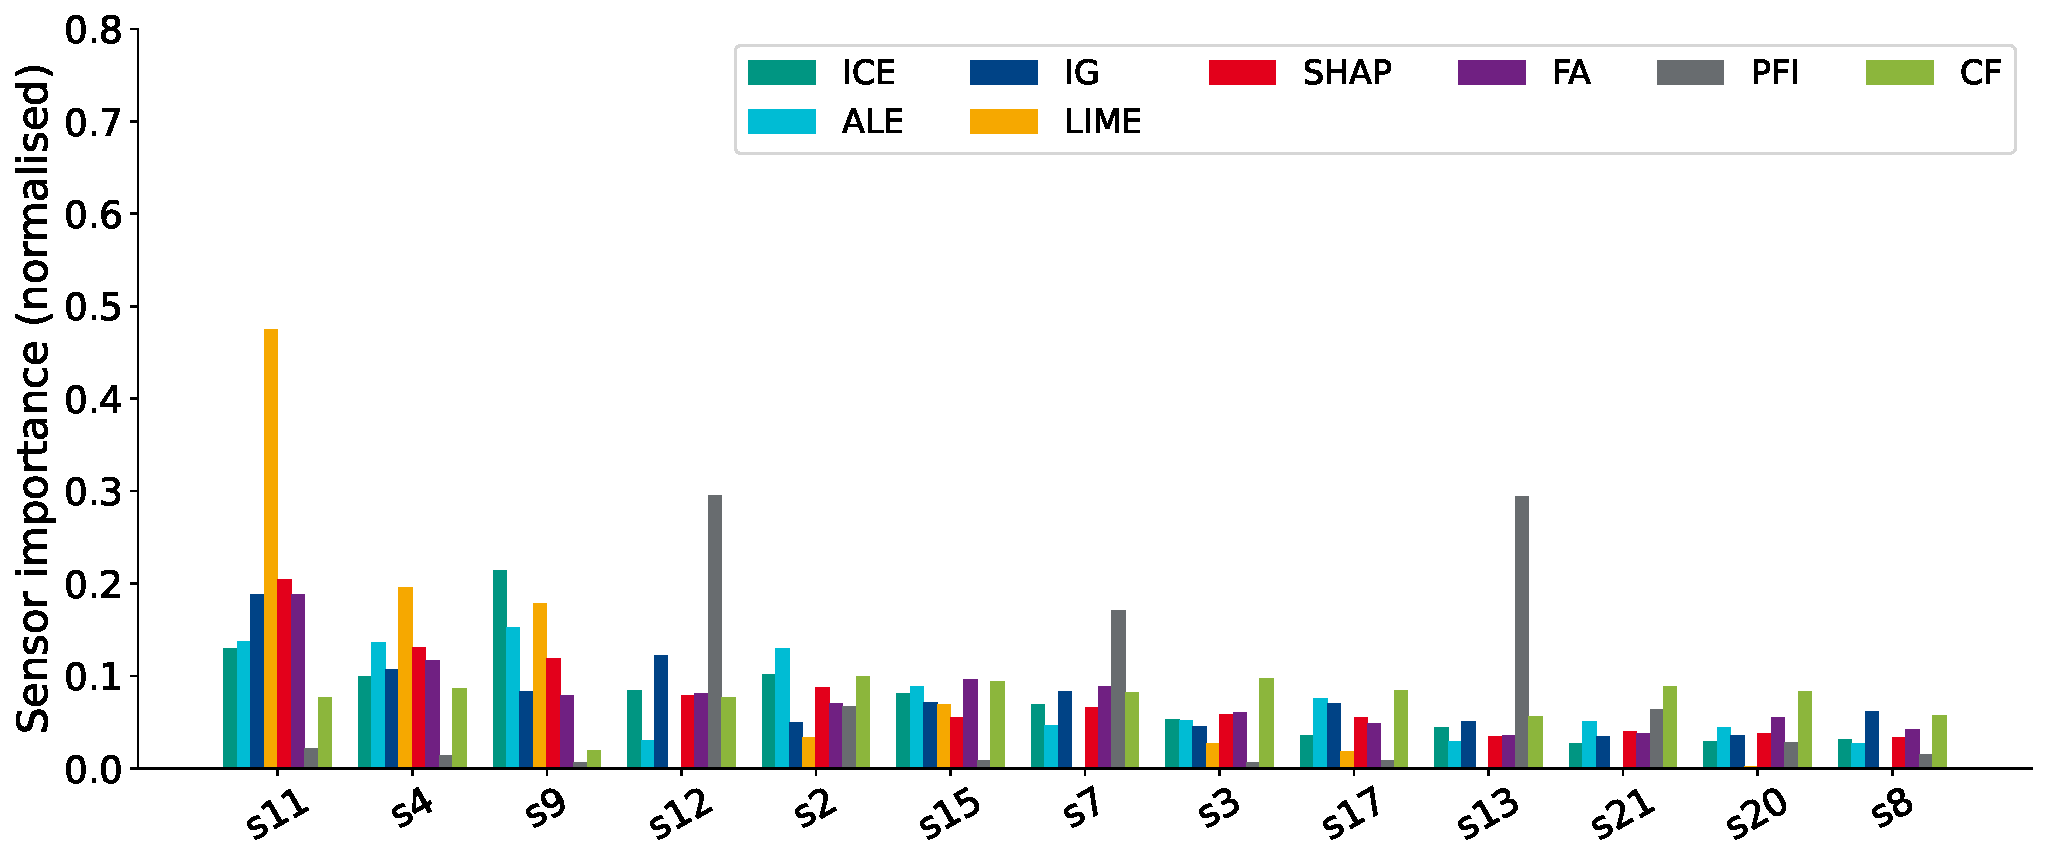
\includegraphics[width=\textwidth]{bilder/Results/compare_methods_all_all.pdf}
    \caption{L1-normalised sensor importance across all eight methods for the model trained on all subsets. Sensors are ordered by decreasing mean importance.}
    \label{fig:compare_all}
\end{figure}

The all-dataset model shows the most agreement across methods. Sesnor s11 is the clear front-runner, IG, SHAP, FA, ALE and ICE all. plcae it first, with normalised importance between 0.10 and 0.19. LIME assigns it roughly 0.48, continuing its pattern of over concentration. Sensors s4 and s9 follow in the secont tier, with s12, s2 and s15 in the middle ground. PFI deviates again, spiking on s12 ($\sim 0.30$) and s13 ($\sim0.30$) while giving s11 minimal importance. CF distributes importance more evenly than in single-dataset cases but still does not match the consensus ranking.

\section{Patterns Across Configuration}
Several patterns hold across all four configuration.

The gradient-based and Shapley-based methods, IG, SHAP and FA, tend to cluster together. they rearely disagree on which sensor is most important ant their normalised magnitudes are usually within a few percentage points of each other. ALE often falls close to this cluster as well. These four methods form what might be called the consensus core of the comparison.

LIME consistently over-concentrates importance onto one or two sensors. It identifies the same top sensor as the consensus core in most cases, but assigns it two to three times the normalised weight. This is a known property of LIME's local linear surrogate fitting: when one feature dominates the local prediction surface, the surrogate can allocate neraly all explanatory weight to it, compressing the contributions of secondary features.

PFI produces isolated spikes on sensors that other methods rank as moderate or low importance. The specific sensor varies by configuration, s8 on FD002, s13 on the all-data model, but the pattern is consistent. These spikes likely reflect individual engines or narrow operating regimes where permuting that sensor causes disproportionate error, inflating the global average.

CF does not produce stable or interpretable rankings in this setting. Its results vary substantially across configurations and rarely agree with the consensus of the other methods. As discurssed in the verification section, counterfactual search is sensitive to the local geometry of the prediction surface and to the permitted perturbation ranges. On a 1D CNN with 13 sensor channels and complex temporal interactions, the search space appears large enough that the results are dominated by search dynamics rathen than meaningful feature effects.

The transisiton from single-dataset to multi-dataset training reveals a shift in which sensor dominate. On FD001alone, s9 lead. On FD002 and multi-dataset configurations, s11 takes over. This shift is discussed further in the context of the underlying physical degradation mechanism in Section~\ref{sec:discussion}.

global comparison

sensor comparison

time comparison

\section{Feature Importance Results per Method}
per method analysis

\section{Comparison}
correlation matrices
feature importance of all methods, summed together -> heat maps

time component 

\section{Discussion}
\label{sec:discussion}



